\section{Visão Geral e Aplicações}

% ==========================================
% minha parte (nicola)
% ==========================================

\begin{frame}{Contexto Histórico}
    \begin{itemize}
        \item O conceito de sensoriamento distribuído surgiu na Guerra Fria com o projeto SOSUS dos EUA, focado na detecção de submarinos soviéticos. %[cite: 1]
        \item Na década de 1980, os programas da DARPA trouxeram os primeiros avanços em direção à computação distribuída moderna. %[cite: 1]
        \item A transição para uso civil ocorreu em 2004 com o surgimento de hardwares específicos (MicaZ, TelosB) e sistemas dedicados como o TinyOS. %[cite: 1]
        \item O experimento na Duck Island (2002) foi um marco prático, utilizando 150 nós para monitorar o clima e o comportamento de pássaros via satélite. %[cite: 1]
    \end{itemize}
\end{frame}

\begin{frame}{Conceitos Fundamentais: A Natureza Ad Hoc}
    \begin{itemize}
        \item As RSSF derivam das redes \textit{Ad Hoc}, formando conexões dinâmicas sem depender de infraestruturas fixas (como roteadores tradicionais). %[cite: 1]
        \item Diferente do modelo ponto-a-ponto, as RSSF focam nos dados coletados, sendo o conteúdo mais importante do que a identidade (ID) do nó que o gerou. %[cite: 1]
        \item Operam em uma topologia altamente dinâmica: a alta taxa de exaustão de baterias exige algoritmos constantes de autoconfiguração. %[cite: 1]
        \item Diferente do Wi-Fi, que foca em alta vazão, as RSSF priorizam a sobrevivência energética e o tráfego convergente para o \textit{sink node} (estação base). %[cite: 1]
    \end{itemize}
\end{frame}

\begin{frame}{Arquitetura de um Nó Sensor (Mote)}
    \begin{columns}
        \begin{column}{0.55\textwidth}
            \begin{itemize}
                \item \textbf{Subsistema de Sensoriamento:} Responsável por converter grandezas físicas (luz, temperatura, aceleração) em sinais digitais via conversores ADC.
                \item \textbf{Subsistema de Processamento:} Unidade central que gerencia o programa e armazena dados em memórias Flash e RAM.
                \item \textbf{Subsistema de Comunicação:} Interface de rádio que utiliza protocolos seriais (como SPI) para trocar informações com o processador.
                \item \textbf{Eficiência Energética:} O processamento local reduz a carga sobre o rádio, que é o componente de maior consumo[cite: 1].
            \end{itemize}
        \end{column}
        
        \begin{column}{0.45\textwidth}
            \begin{figure}
                \centering
                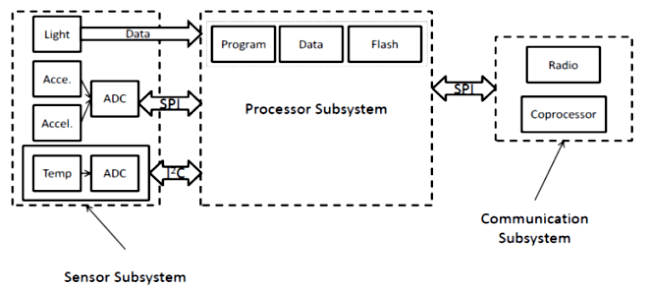
\includegraphics[width=\textwidth]{figuras/arquitetura.png}
                \caption{Arquitetura modular de um nó sensor.}
                \vspace{0.1cm}
                {\tiny Fonte: ResearchGate (Adaptado de Silva et al.)}
            \end{figure}
        \end{column}
    \end{columns}
\end{frame}

% ==========================================
% parte waldemar
% ==========================================

